\section{网络编码与TCP/NC协议}

%%==========第一节==========
\subsection{网络编码理论基础}
%%网络编码概念
\begin{frame}[t]
	\frametitle{网络编码概念}
	R.Ahlswede等人在论文“Network Information Flow\footfullcite{Ahlswede2000}”首次提出\emph{网络编码}概念。
	网络编码建立在一个简单而广泛的概念的基础上:
	\begin{block}{网络编码}
		\footnotesize
		在包交换网络中,
		中间节点不仅仅是简单地路由转发接收到的数据包,
		而是对它们进行一些函数操作并计算、转发操作结果。
	\end{block}
	\vspace{1em}
	运用网络编码可以提高网络吞吐率、均衡网络负载和提高网络带宽利用率。
	\\
	我们以简单的蝶形网络为例,说明Network Coding的基本原理。
	\note{
		在接收TCP/NC之前,先简单介绍一下网络编码的相关知识。
	}
\end{frame}
%%网络编码的一个简单例子
\begin{frame}[t]
	\frametitle{网络编码的一个简单例子}
	\vspace{-1.5em}
	\begin{figure}[t]
		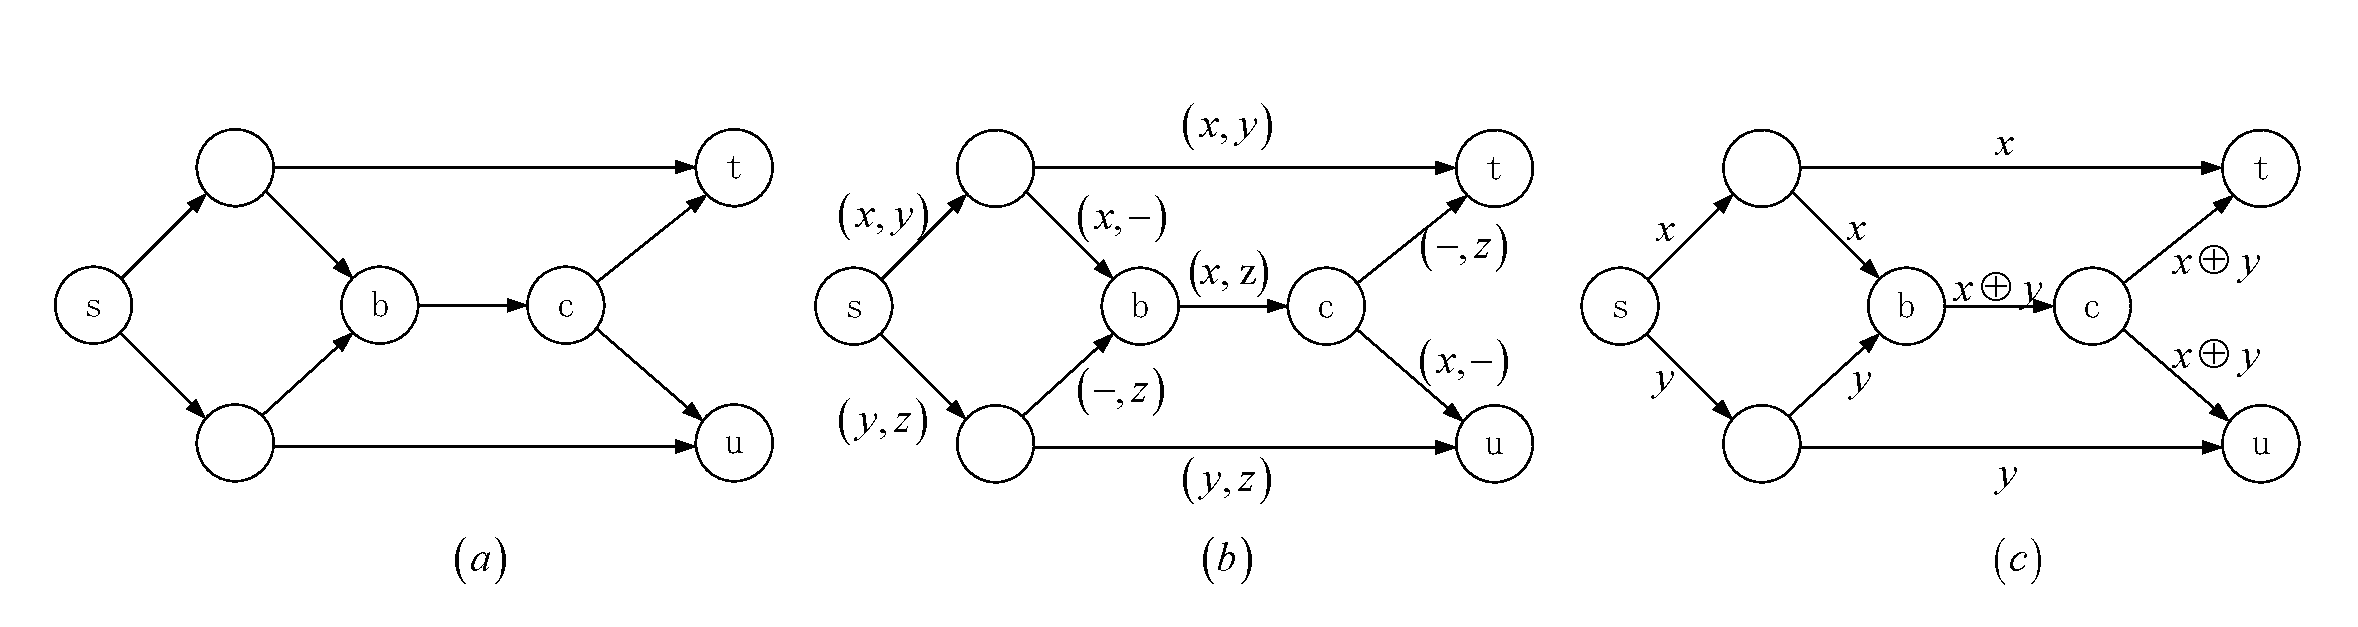
\includegraphics[height=2.5cm]{../figures/butter.eps}
		\caption{蝶形网络}
		\label{fig:butter}
	\end{figure}
	\vspace{-1em}
%	图\ref{fig:butter}为一个包交换模型。
	图\ref{fig:butter}(b)为传统的路由算法,
	其多播吞吐量为1.5。
	图\ref{fig:butter}(c)为应用了网络编码的路由算法,
	其多播吞吐量为2,且是理论上最大的网络多播吞吐量。
	\begin{mytheorem}
	一个网络的最大多播吞吐量取决于分割源节点和目的节点的最小割集\supercite{Ahlswede2000}。
	\end{mytheorem}

\end{frame}
%%线性网络编码
\begin{frame}[t,allowframebreaks]
	\frametitle{线性网络编码}
	%%第一帧
	令$\left(p_1,p_2,\dots,p_r\right)^{T}$表示进入源节点$s$的数据包${{\rm X}_{{\rm I}\left( s \right)}}$。
	每个数据包$p_i$都是$\mathbb{F}_{q}$上长度为$m$的矢量。
	我们可以用一个定义在$\mathbb{F}_{q}$上的$r \times m$矩阵来表示${\rm X}_{{\rm I}\left( s \right)}$,
	该矩阵的第$i$行是$p_{i}$。
	\\
	\vspace{1em}
	本地编码函数是$\mathbb{F}_{q}$上的线性函数,即任意中间节点$v$输出的数据包列向量${\rm X}_{{\rm O}\left( v \right)}$与其接收到的数据包列向量${\rm X}_{{\rm I}\left( v \right)}$之间的关系可以用以下线性方程组表示:
	\begin{equation}\label{eq:xianxingfangchengzu}
	{\rm X}_{{\rm O}\left( v \right)}={\rm L}_{v}{\rm X}_{{\rm I}_{\left( v \right)}}
	\end{equation}
	其中,${\rm L}_{v}$是定义在${\mathbb{F}}_{q}$上的系数矩阵。
	考虑到网络中只允许线性操作,
	因此任意边上传输的数据包都是原数据包$p_{1},p_{2},\dots,p_{r}$的线性组合。
	\newpage
	%%第二帧
	也就是$\forall v \in V$,有
	\begin{equation}\label{eq:xishujuzheng}
	{\rm X}_{{\rm I}\left( v \right)}=G_{v}\left[ {\begin{array}{*{20}{c}}
		{{p_1}}\\
		\vdots \\
		{{p_r}}
		\end{array}} \right]
	\end{equation}
	\begin{columns}[onlytextwidth]
		\vspace{3em}
		\begin{column}{0.6\textwidth}
			其中,$G_{v}$是定义在$\mathbb{F}_{q}$上的系数矩阵,
			也称为$v$的全局转移矩阵。
			${\rm G}_{v}$的每一行都对应一条边$e \in {\rm I}_{\left( v \right)}$,
			称为边$e$的全局编码向量。
			图\ref{fig:zhuanyi}为标示了本地转移矩阵的蝶形网络,
			我们可以得到在目的节点$t$和$u$的全局转移矩阵为:
		\end{column}
		\begin{column}{0.4\textwidth}
			\vspace{-1em}
			\begin{figure}
				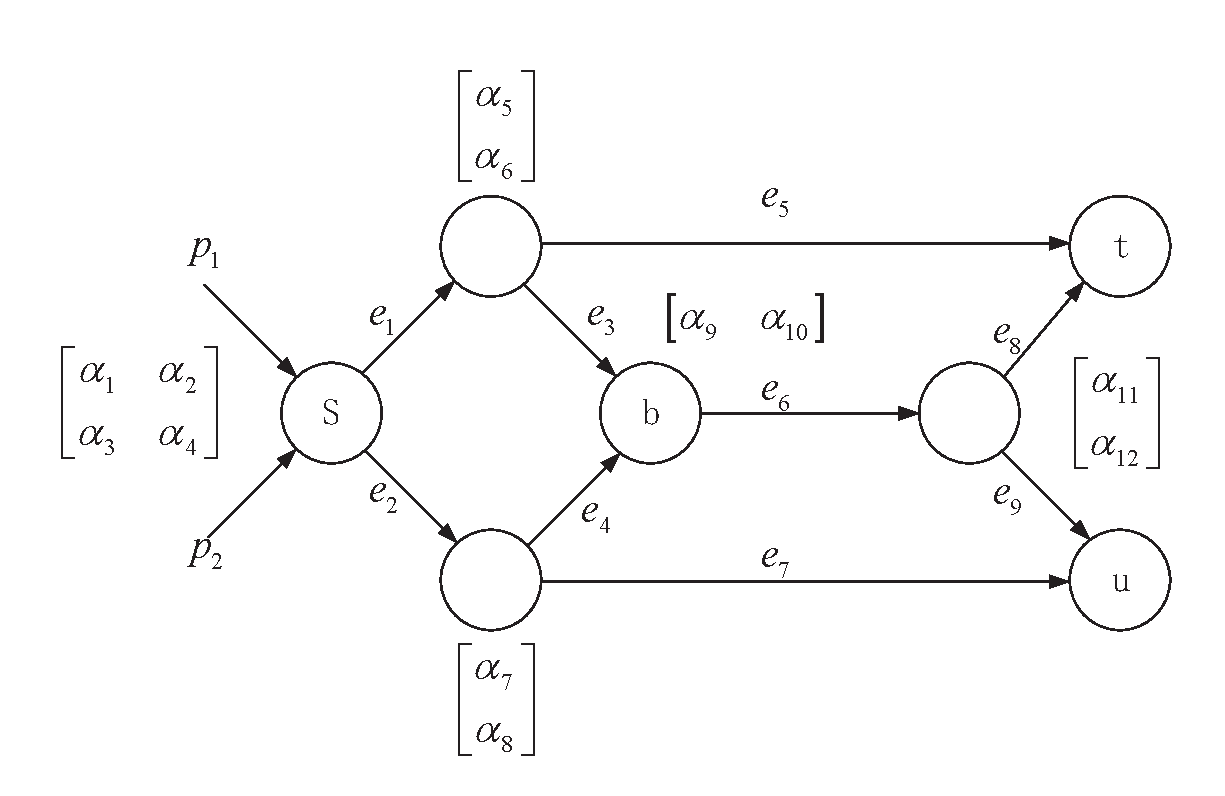
\includegraphics[height=3cm]{../figures/zhuanyi.eps}
				\caption{标注了转移矩阵的蝶形网络}
				\label{fig:zhuanyi}
			\end{figure}
		\end{column}
	\end{columns}
	
	\newpage
	\begin{eqnarray}\label{eq:quanjuzhuanyi}
	{G_t} = \left[ {\begin{array}{*{20}{c}}
		{{\alpha _1}{\alpha _5}}&{{\alpha _2}{\alpha _5}}\\
		{{\alpha _1}{\alpha _6}{\alpha _9}{\alpha _{11} }+{\alpha _3}{\alpha _7}{\alpha _{10}}{\alpha _{11} }}&{{\alpha _2}{\alpha _6}{\alpha _9}{\alpha _{11}}+{\alpha _4}{\alpha _7}{\alpha _{10}}{\alpha _{11}}}
		\end{array}} \right] \nonumber \\
	{G_u}= \left[ {\begin{array}{*{20}{c}}
		{{\alpha _1}{\alpha _6}{\alpha _9}{\alpha _{12} }+{\alpha _3}{\alpha _7}{\alpha _{10}}{\alpha _{12} }}&{{\alpha _2}{\alpha _6}{\alpha _9}{\alpha _{12}}+{\alpha _4}{\alpha _7}{\alpha _{10}}{\alpha _{12}}}\\
		{{\alpha _3}{\alpha _8}}&{{\alpha _4}{\alpha _8}}
		\end{array}} \right]
	\end{eqnarray}
	对于目的节点$t$来说,
	当且仅当$\left|{\rm I}\left(t\right)\right| \times r$阶全局转移矩阵$G_{t}$的秩为$r$时,
	$t$才能恢复出$\left(p_1,p_2,\dots,p_r\right)$中的所有元素。
	因为只有$G_t$满秩时,
	才存在满足${G_t}^{-1}G_t={\rm I}_r$的左逆矩阵,
	其中${\rm I}_r$是$r \times r$阶单位矩阵。
	只需$G_{t}$满秩,
	而不要求$G_{t}$是可求逆的方阵。
	目的节点$t$可以通过计算${G_t}^{-1}{\rm X}_{{\rm I}\left(t\right)}$得到$\left(p_1,p_2,\dots,p_r\right)^{T}$。

	\note{
		换句话说,$v$输出的每个数据包( ${\rm X}_{{\rm O}\left( v \right)}$的一个分量)都可以看做是进入$v$的多个数据包在$\mathbb{F}_{q}$上的线性组合。
	}
\end{frame}
%%两种网络编码
\begin{frame}[t,allowframebreaks]
	\frametitle{Batch Coding和Pipeline Coding}
	将网络编码应用于提升有损链路的吞吐率,
	其应用方式主要有两种:Batch Coding和Pipeline Coding。
	\begin{block}{Batch Coding}
		定义\emph{generation}为数据包的集合,作为编解码的整体。
		源节点和网络中的中间节点在同一个\emph{generation}上进行编码,
		目的节点只有在收到足够多的编码报文后,
		才能一次性解出这一个\emph{generation}中的所有原始报文。
	\end{block}
	假设$p_1,p_2,\dots$为原始数据包,\emph{k}为\emph{generation}的大小,
	第$i^{th}$个\emph{generation}产生的一个编码包可以被表示为:
	\begin{equation}\label{eq:batch-pkt}
	c = \sum\limits_{j = 1}^k {{e_j}{p_{i \times k + j}}}
	\end{equation}
	\newpage
	\begin{block}{Pipeline Coding}
		无需等待一个\emph{generation}满秩,
		每当一个数据报文来之后,
		就会产生一个编码包。
		目的节点会逐步解出原始报文。
	\end{block}
	Pipeline Coding的编码函数为:
	\begin{equation}\label{eq:pipelinecoding}
	c = \sum\limits_{j = 1}^m {{e_j}{p_{i \times k + j}}}
	\end{equation}
	其中\emph{m}表示目前在编码缓存中数据包的个数。
	图\ref{fig:codingMechanism}为两种编码方式示例,
	其中冗余度都为1.25,即每发送4个报文发送一个冗余包。
	\newpage
	 \begin{figure}
		\centering
		\begin{boxedminipage}{1\textwidth}
		\subfloat[]{
			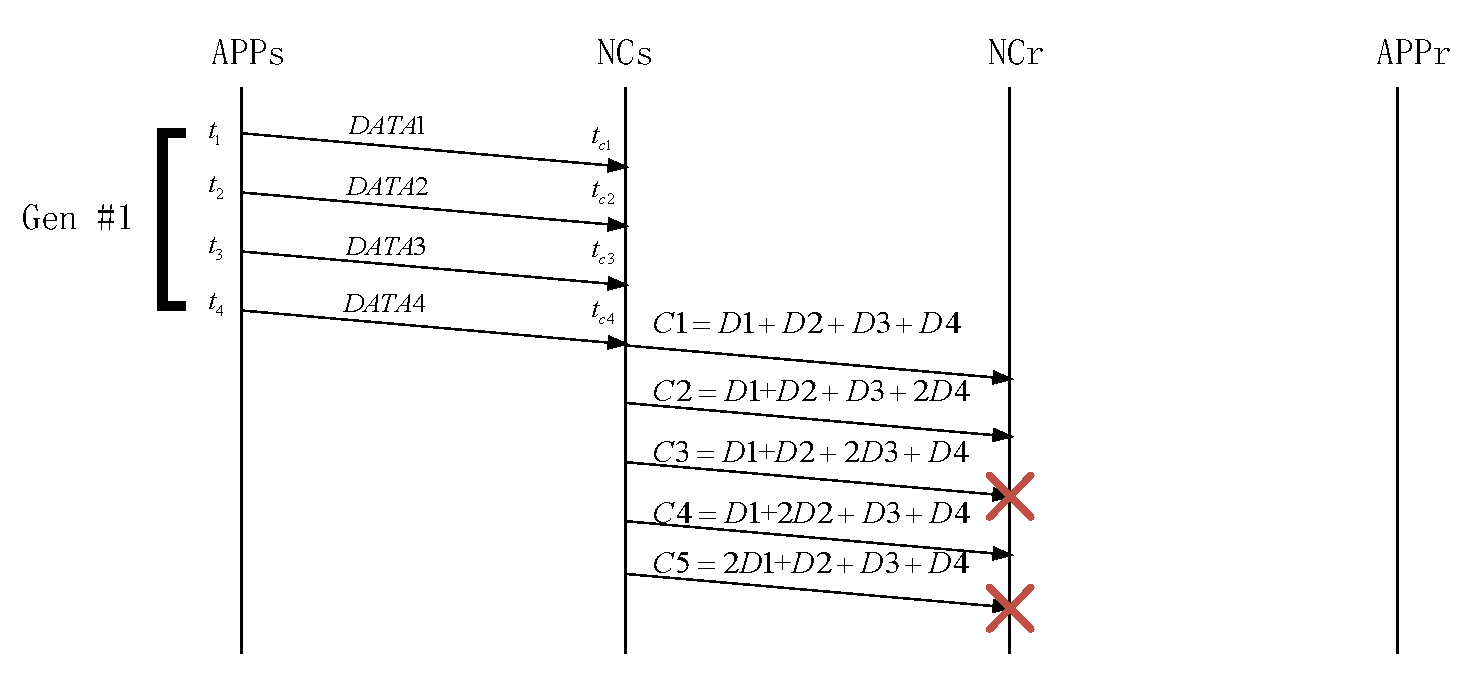
\includegraphics[width=2in]{../figures/batchundecode.eps}
			\label{fig:batchcoding}
		}
		\hspace{6em}
		\subfloat[]{
			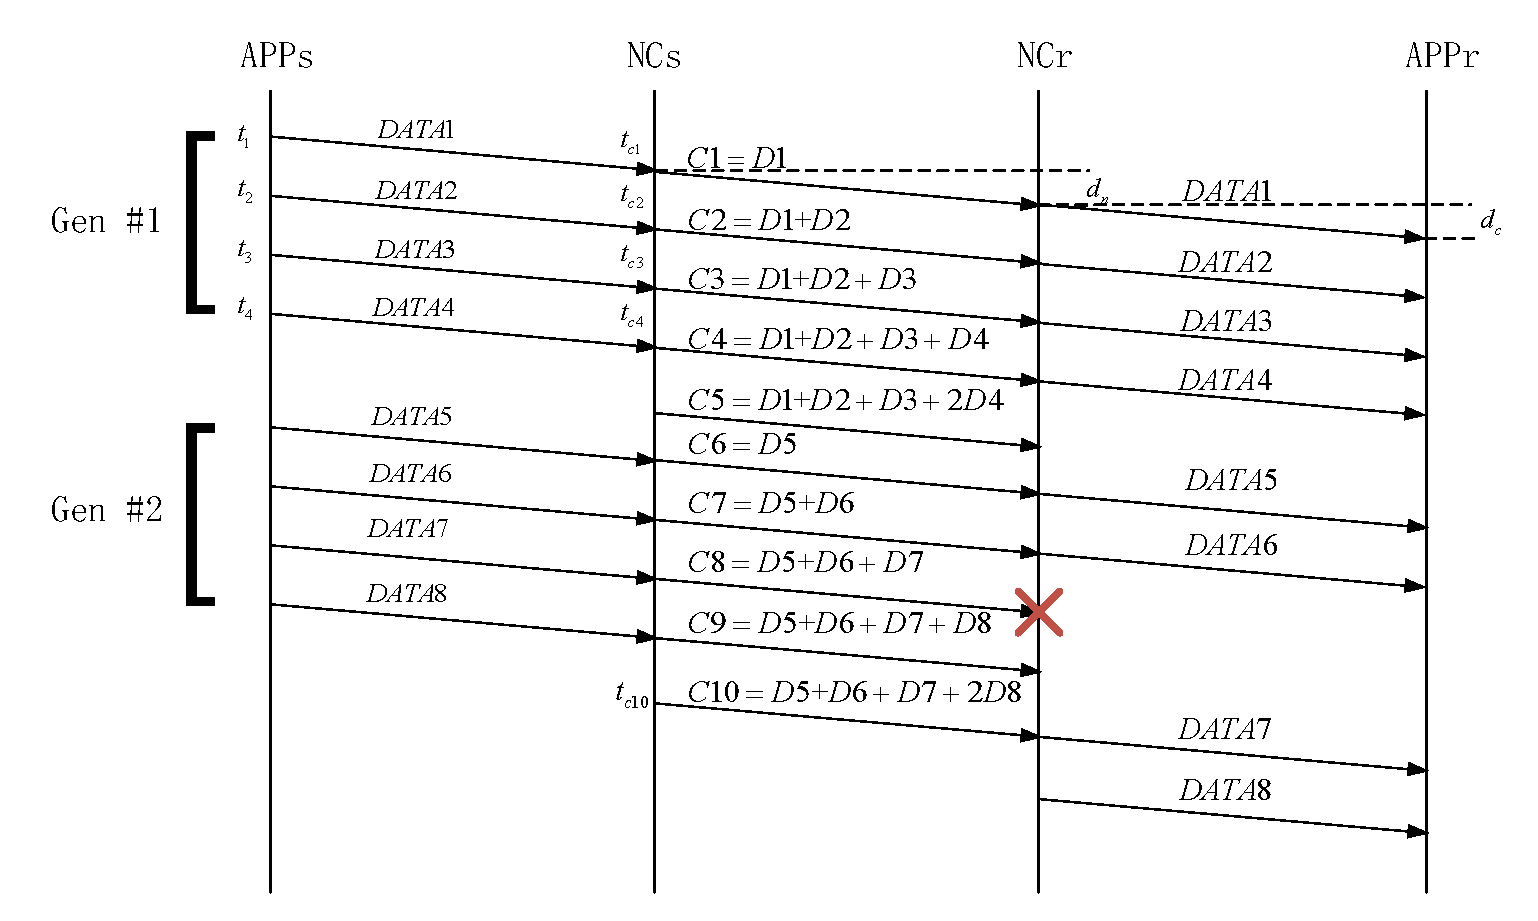
\includegraphics[width=2in]{../figures/pipeline.eps}
			\label{fig:pipelinecoding}
		}
		\end{boxedminipage}
		\caption{\small (a) Batch Coding ~~ (b) Pipeline Coding}
		\label{fig:codingMechanism}
	\end{figure}
	采用Pipeline Coding的优点:解码时延更低。
	\note{
		由于每个编码数据包都是同一个\emph{generation}的数据包的线性组合,
		在源节点就引入了一个延时。
		换句话说,
		同一个\emph{generation}里面前面的报文需要等后面的报文,
		直到这个\emph{generation}满秩候,才可进行编码。
		在目的节点处,
		同一个\emph{generation}的报文,
		要么都解码,
		要么一个都解不出。
		i表示第i个\emph{generation}。
	}
\end{frame}

%%==========第二节==========
\subsection{TCP/NC协议}
%%ACK On degree of freedom
\begin{frame}[t,allowframebreaks]
	\frametitle{ACK On degree of freedom}
	TCP、ARQ协议中的ACK都是对原始数据包的确认,
	\emph{ACK On degree of freedom}\footfullcite{4595268}则对\emph{自由度}进行确认。
	\begin{myDef}[See a packet]\label{def:seepkt}
	如果一个节点根据现有的信息可以计算出如\textbf{\emph{$\left(p+q\right)$}}形式的线性组合,
	那么我们就说这个节点“\textbf{see packet \emph{$p$}}”。
	其中\textbf{$q$}本身就是只包含序号比$p$大的报文的线性组合。
	解码出某个报文也算作是“\textbf{see a packet}”,此时\textbf{$q=0$}。
	\end{myDef}
	接收端如果\emph{see packet p},那么就需要对\emph{p}进行ACK。
	表\ref{tab:ack-on-degree-of-freedom}为\emph{ACK on degree of freedom}的例子。
	\newpage
	\vspace*{-3em}
	\begin{table}  
	\centering  
	\fontsize{6.5}{8}\selectfont  
	\begin{threeparttable}  
		\caption{\emph{ACK on degree of freedom} 例子}  
		\label{tab:ack-on-degree-of-freedom}  
		\begin{tabular}{c|c|c|c|c|c}  
			\toprule  
			\multirow{2}{*}{Time} &\multirow{2}{*}{Sender's queue} & \multirow{2}{*}{Transmitted packet} & \multirow{2}{*}{Channel state}&  
			\multicolumn{2}{c}{ Destination Node \emph{A}}\cr  
			\cmidrule(lr){5-6}  
			\hspace{1cm}&\hspace{1cm}&\hspace{1cm}&\hspace{1cm}&Decoded&Seen but not decoded\cr  
			\midrule  
			1&$p_{1}$&$p_{1}$&$\nrightarrow A$&\hspace{1cm}&\hspace{1cm}\cr
			\hline  
			2&$p_{1}$,$p_{2}$&$p_{1} \oplus p_{2}$&$\rightarrow A$&\hspace{1cm}&$p_{1}$\cr 
			\hline 
			3&$p_{2}$,$p_{3}$&$p_{2} \oplus p_{3}$&$\rightarrow A$&\hspace{1cm}&$p_{1}$,$p_{2}$\cr
			\hline  
			4&$p_{3}$,$p_{4}$&$p_{3} \oplus p_{4}$&$\nrightarrow A$&\hspace{1cm}&$p_{1}$,$p_{2}$\cr
			\hline  
			5&$p_{3}$,$p_{4}$,$p_{5}$&$p_{3} \oplus p_{4} \oplus p_{5}$&$\rightarrow A$&\hspace{1cm}&$p_{1}$,$p_{2}$,$p_{3}$\cr
			\hline  
			6&$p_{4}$&$p_{4}$&$\rightarrow A$&$p_{4}$&$p_{1}$,$p_{2}$,$p_{3}$,$p_{5}$\cr
			\hline
			7&$p_{5}$&$p_{5}$&$\rightarrow A$&$p_{1}$,$p_{2}$,$p_{3}$,$p_{4}$,$p_{5}$&\hspace{1cm}\cr    
			\bottomrule  
		\end{tabular}  
	\end{threeparttable}  
	\end{table}
	优点:发送端可以减小发送队列的长度。
\end{frame}

\begin{frame}[t]
	\frametitle{TCP/NC概述}
	为了提高标准TCP在有损信道环境下的性能,
	Sundararajan等人提出了TCP/NC。
	将网络编码和TCP结合起来,
	在发送端冗余编码,
	掩盖链路中出现的丢包。
	\\
	其关键点有:
	\begin{block}{TCP/NC关键点}
		\begin{enumerate}
			\item 在发送端的TCP层和NC层插入一个网络编码层,
			在编码层对数据包进行线性网络编码。
			\item 利用\emph{ACK On degree of freedom}的概念,
			重新定义TCP中ACK的概念。
			\item 发送端通过冗余编码来补偿链路中出现的丢包
		\end{enumerate}
	\end{block}
\end{frame}

%%TCP/NC框图
\frame{
	\frametitle{TCP/NC框图}
	\begin{columns}[onlytextwidth]
		\hspace{-3.0em}
		\begin{column}{0.45\textwidth}
			\begin{figure}
      		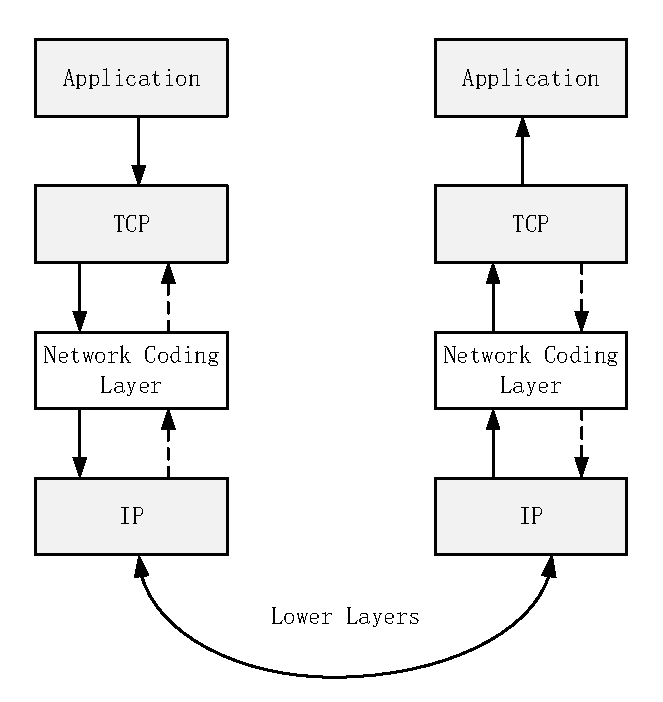
\includegraphics[height=5cm]{../figures/tcpnc.eps}
      		\caption{TCP/NC结构框图}
      		\label{fig:tcpnc}
      	\end{figure}
      	\end{column}
      	\begin{column}{0.65\textwidth}
      		\footnotesize
      		\begin{block}{NC层发送端}
      			\begin{enumerate}
      				\item 接收TCP层的数据包,
      				根据编码窗口和冗余因子对数据包进行线性组合,
      				然后发往IP层。
      				\item 处理接收端回复的ACK报文,
      				并据此删除编码队列的报文。
      			\end{enumerate}
      		\end{block}
      		\begin{block}{NC层接收端}
      			\begin{enumerate}
      				\item 接收IP层传上来的编码包,
      				并进行解码运算。
      				如果有新的报文被看到,
      				回复发送端ACK报文;
      				如果有新的原始数据包被解码,
      				将其传给上层TCP。
      				\item 拦截上层TCP下来的ACK报文。
      			\end{enumerate}
      		\end{block}
      \end{column}
  \end{columns}
  \note{
  }
}

%\frame{
%	\frametitle{Seen Packet}
%	\vspace{-2em}
%	\begin{myDef}[See a packet]\label{def:seepkt}
%		如果一个节点根据现有的信息可以计算出如\textbf{\emph{$\left(p+q\right)$}}形式的线性组合,
%		那么我们就说这个节点“\textbf{see packet \emph{$p$}}”。
%		其中\textbf{$q$}本身就是只包含序号比$p$大的报文的线性组合。
%		解码出某个报文也算作是“\textbf{see a packet}”,此时\textbf{$q=0$}。
%	\end{myDef}
%	\vspace{+1em}
%	例如,接收端收到编码包$C\left[1\right]=p_1+p_2+p_3+p_4$,
%	由定义\ref{def:seepkt}可知,
%	接收端看到了报文$p_1$。
%	如果再次接收到$C\left[2\right]=p_1+2p_2+3p_3+p_4$,
%	由$C\left[2\right] - C\left[1\right] = p_2+p_3$,
%	由定义\ref{def:seepkt}可知,接收端看到了报文$p_2$。
%	接收端对于看到的每个报文,
%	都会回复给发送端一个ACK。
%	
%}
%%编解码示例
\begin{frame}[t]
	\frametitle{编解码示例}
 	\begin{columns}[t,onlytextwidth]
    	\hspace{-2.0em}
    	\begin{column}{0.55\textwidth}
    		\vspace{-2em}
    		\begin{figure}
    			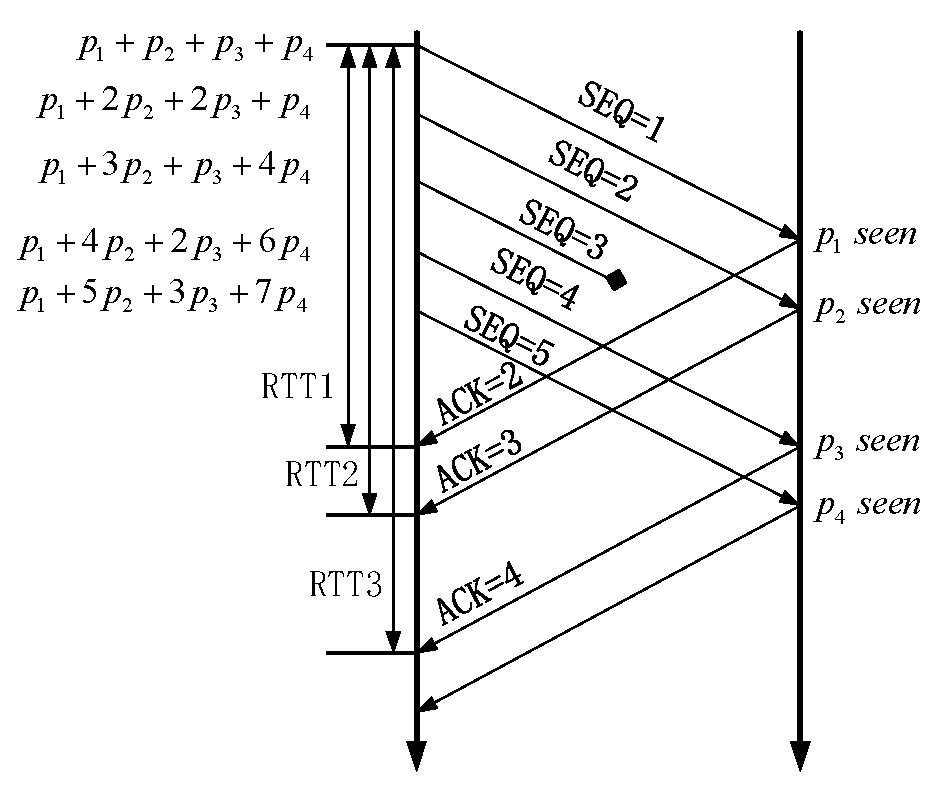
\includegraphics[height=5cm]{figures/encodingexp.eps}
    			\caption{编码发送示例}
    			\label{fig:codingexp}
    		\end{figure}
    	\end{column}
    	\hspace{2.5em}
    	\begin{column}{0.45\textwidth}
    		图\ref{fig:codingexp}所示为冗余度1.25时编码发送的一个示例。\\
    		\vspace{1em}
    		尽管$SEQ=3$丢失,
    		但是接收端在收到$SEQ=4$的编码包后,
    		看到了报文$p_3$,
    		所以回复给发送端的是$ACK=4$。
    		在收到冗余报文$SEQ=5$后,
    		看到了$p_4$,
    		同时也将$p_1 \sim p_4$全部解出。\\
    		\vspace{1em}
    		链路的丢包在发送端的TCP层看来仅仅是RTT的增大。
    	\end{column}
	\end{columns}
\end{frame}

\begin{frame}
	\frametitle{冗余度}
	TCP/NC能够抵抗链路丢包的关键是发送端进行了冗余编码。
	冗余度决定了TCP/NC发送冗余包的多少。
	\\
	理论上,当链路的丢包率为$\rho$时,设置的冗余度\emph{R}应该为
	\begin{equation}\label{eq:redundancy}
	R=\dfrac{1}{1 - \rho}
	\end{equation}
	此时,链路中出现的丢包刚好全部被冗余包补偿。
\end{frame}


\frame{
\frametitle{传输时延 }
\vspace{-1em}
\begin{myDef}[传输时延]\label{def:shiyan}
   	如果源节点产生数据报文$pkt_i$的时间为$t_{s_i}$,
   	目的节点将数据报文$pkt_i$交付给上层时间为$t_{r_i}$,
   	定义数据包的传输时延为$delay_i=t_{r_i} - t_{s_i}$。
\end{myDef}
\begin{block}{解码导致的时延}
  	TCP/NC的基本思想是利用发送端的编码将链路的丢包问题后延,
  	当发送端的冗余包足够弥补链路丢包后,
  	丢包就被掩盖。
  	带来的问题是数据包的传输时延变大。
  	以图\ref{fig:codingexp}为例,
  	如果补偿$SEQ=2$的冗余包为$SEQ=7$,
  	那么$p_2$需要等到$SEQ=7$才能被接收端的NC层交付给上层TCP。
  	那么$p_2$的传输时延为$delay_2 = t_{r_7} - t_{s_2}$。
   \end{block}

\note{
(介绍PPT后),本文后面的实验就是基于BVH的,不可变形的三角网格。//现在研究较多的是连续的可变形的碰撞检测布料模拟头发模拟等。
}
}
%
%  \frame{
%    \frametitle{基于~BVH~的碰撞检测算法}
%    \begin{columns}[onlytextwidth]
%      \begin{column}{0.35\textwidth}
%        \vspace{-1.5em}
%        \begin{figure}[htbp]
%            \begin{center}
%            \begin{boxedminipage}{1\textwidth}
%            \subfloat{\label{lbl:bvh-bunny-center-0.png}}
%              {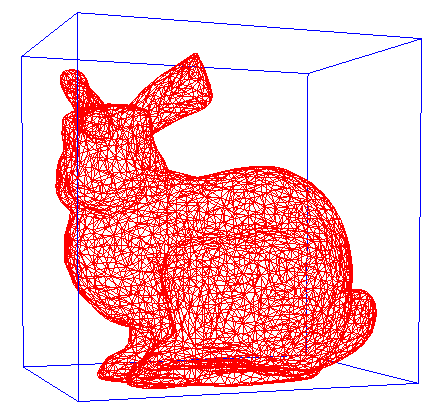
\includegraphics[height=1.4cm]{bvh-bunny-center-0.png}}
%            \subfloat{\label{lbl:bvh-bunny-center-1.png}}
%              {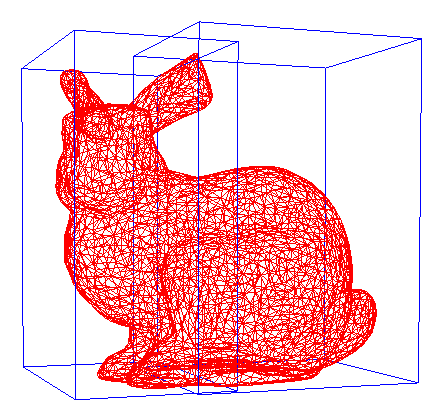
\includegraphics[height=1.4cm]{bvh-bunny-center-1.png}}
%            \\
%            \subfloat{\label{lbl:bvh-bunny-center-2.png}}
%              {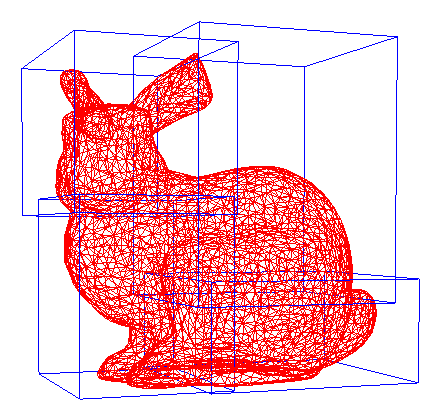
\includegraphics[height=1.4cm]{bvh-bunny-center-2.png}}
%            \subfloat{\label{lbl:bvh-bunny-center-3.png}}
%              {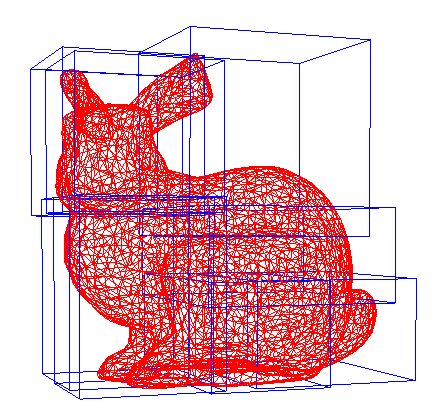
\includegraphics[height=1.4cm]{bvh-bunny-center-3.png}}
%            \\\hspace{0.5cm}
%            \subfloat{\label{lbl:bvh-bunny-center-4.png}}
%              {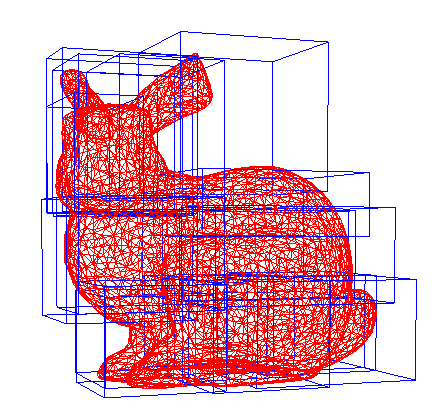
\includegraphics[height=1.5cm]{bvh-bunny-center-4.png}}
%            \subfloat{\label{lbl:bvh-bunny-center-5.png}}
%              {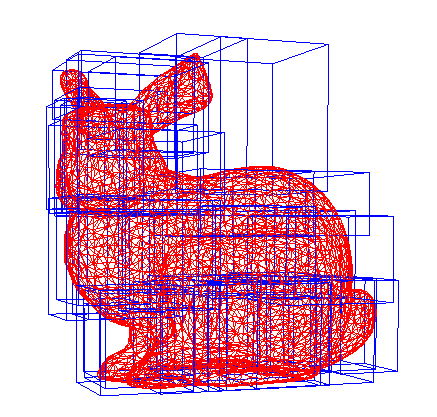
\includegraphics[height=1.5cm]{bvh-bunny-center-5.png}}
%            \\
%            \subfloat{\label{lbl:bvh-bunny-center-6.png}}
%              {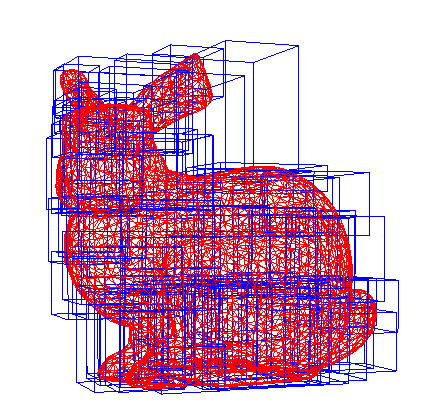
\includegraphics[height=1.5cm]{bvh-bunny-center-6.png}}
%            \subfloat{\label{lbl:bvh-bunny-center-7.png}}
%              {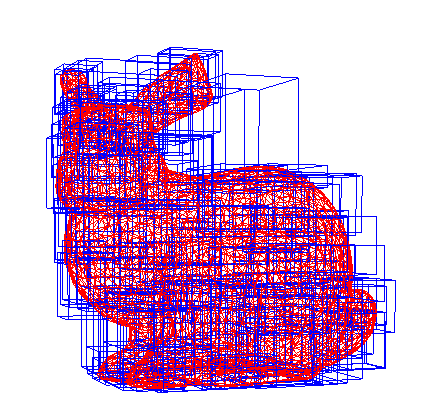
\includegraphics[height=1.5cm]{bvh-bunny-center-7.png}}
%            \end{boxedminipage}
%            \vspace{-0.5em}
%          \caption{八层~BVH~示例}
%          \label{lbl:bvh-example}
%          \end{center}
%          \end{figure}
%      \end{column}
%      \hspace{0.5em}
%      \begin{column}{1.2\textwidth}
%      \vspace{0.2em}
%         \scalebox{0.5}{
%              \begin{minipage}{1.0\textwidth}
%      \vspace{-2em}
%           \begin{algorithm}[H]
%              \caption{自顶向下层次遍历~BVH~}
%              \label{alg:traverse-bvh-tree}
%              \begin{algorithmic}[1]
%              \Require
%              两个~BVH~树的根节点~$node_1$,$node_2$
%              \Ensure
%              模型是否相交
%              \Function {TraverseBVHTree}{$node_1, node_2$}
%                \If{$node_1.bv \cap node_2.bv = \emptyset$}
%                  \State \Return{\textbf{False}}
%                  \Comment{包围体重合测试, 包围体不相交直接返回}
%                \Else
%                    \If {$node_1.children = \emptyset$}
%                         \If {$node_2.children = \emptyset$}
%                         \State \Comment{最底层叶子节点原生几何相交测试}
%                         \State \Return {\Call{CheckIntersection}{$node_1.primitives, node_2.primitives$}}
%                         \Else
%                            \ForAll {$child \in node_2.children$}
%                            \State \Call{TraverseBVHTree}{$node_1, child$} \Comment{递归调用}
%                            \EndFor
%                         \EndIf
%                    \Else
%                         \ForAll {$child \in node_1.children$}
%                         \State \Call{TraverseBVHTree}{$child, node_2$}  \Comment{递归调用}
%                         \EndFor
%                    \EndIf
%                \EndIf
%              \EndFunction
%              \end{algorithmic}
%              \end{algorithm}
%              \end{minipage}
%            }
%      \\
%      \scriptsize \hspace{1em}代价函数: $T_{cost} = n_v * C_v + n_p * C_p + (n_u * C_u)$(运动)
%      \end{column}
%    \end{columns}
%    \note{
%      基于包围体树的碰撞检测算法, 一般首先都会初始化环境然后构建层次结构的包围体树,碰撞检测时从顶层开始逐渐往下层遍历,到最底层叶子节点后开始三角网格模型相交测试,
%      当发现三角网格相交后立即终止遍历,确定模型发生碰撞。
%      评价碰撞检测算法的指标一般用上面这个公式来衡量,其中nv和 np分别表示参与包围体节点相交测试的数量和参与原始几何相交测试的数量,Cv和 Cp则表示相应的平均测试耗费的代价。
%      当在运动场景时还需要加上nu和 Cn就是模型旋转或者运动后包围体更新的数量和更新的代价。
%      本文算法就是尽早发现包围体不相交的情况,减少np和cp的数量。
%    }
%}
